\NeedsTeXFormat{LaTeX2e}
\documentclass[12pt,oneside,a4paper]{article}
\usepackage[left=2cm, right=2cm, top=1cm, bottom=2cm]{geometry}
\usepackage{amsmath,amsfonts,amssymb,amsthm}
\usepackage[utf8]{vietnam}
\usepackage{graphicx}
\usepackage[american]{circuitikz}
\usepackage{float}
\usepackage{mathptmx}
\usepackage{multicol}
\usepackage{enumitem} 
\usepackage{tasks} 
\usepackage{booktabs}
\usepackage{array}
\usepackage{caption}
\usepackage{hyperref}

\everymath{\displaystyle}
\theoremstyle{definition}
\newtheorem{bt}{} 
\renewcommand{\thebt}{\textbf{\large Q\arabic{bt}}} 

\newcommand{\bb}[1]{\mathbb{#1}}

\newlist{questions}{enumerate}{1}
\setlist[questions]{label=\textbf{Q$_{\mathbf{\arabic*}}$:}, leftmargin=4em}

\settasks{label=\textbf{\Alph*.}, label-width=1.5em, item-indent=7mm}

\begin{document}
	\renewcommand{\figurename}{Figure}
	\renewcommand{\tablename}{Table}
	
	\begin{center}
		\textbf{\Large EXPERIMENT 1}
		
		\vspace{0.5cm}
		\textbf{{\Large MEASUREMENT OF RESISTANCE, CAPACITANCE,}}
		
		\vspace{0.1cm}
		\textbf{{\Large INDUCTANCE AND RESONANT FREQUENCIES}}
		
		\vspace{0.1cm}
		\textbf{{\Large OF RLC CIRCUIT USING OSCILLOSCOPE}}
	\end{center}
	
	\vspace{0.5cm}
	
	\noindent
	\begin{minipage}[t]{0.5\textwidth}
		\vspace{0.5cm}
		\textbf{Class: IT-E10 02} \\[0.2cm]
		\textbf{Group: 3} \\[0.2cm]
		\textbf{Name: Nguyễn Trọng Phúc Anh} \\[0.2cm]
		\textbf{Student ID: 202516522}
	\end{minipage}%
	\begin{minipage}[t]{0.5\textwidth}
		\vspace{0pt}
		\centering
		\textit{\textbf{Verification of the instructors}} \\[0.2cm]
		\begin{tabular}{|p{3.5cm}|p{3.5cm}|}
			\hline
			& \\[2.5cm]
			\hline
		\end{tabular}
	\end{minipage}
	
	\vspace{0.8cm}
	
	\section*{1. THEORETICAL BACKGROUND}
	
	\subsection*{1.1. RLC Circuit}
	An RLC circuit (also known as a resonant circuit or a tuned circuit) is an electrical circuit consisting of a resistor ($R$), an inductor ($L$), and a capacitor ($C$), connected in series or in parallel. Every RLC circuit consists of two main components: a power source and a resonator (series LC or parallel LC).
	\begin{center}
		\begin{circuitikz}[american]
			\draw (0,0) to[sV, l=$E$] (0,2.5)
			to[R, l=$R$] (5,2.5)
			to[L, l=$L$] (5,0)
			to[C, l=$C$] (0,0);
			
			\draw (7.5,0) to[sV, l=$E$] (7.5,2.5)
			to[R, l=$R$] (10.5,2.5)
			to[short] (12.5,2.5);
			\draw (10.5,2.5) to[C, l=$C$] (10.5,0);
			\draw (12.5,2.5) to[L, l=$L$] (12.5,0);
			\draw (12.5,0) to[short] (7.5,0);
		\end{circuitikz}
		\captionof{figure}{\textit{Series (left) and parallel (right) RLC circuit }}
	\end{center}
	The undamped resonance or natural angular frequency of an $LC$ circuit (in $\text{rad/s}$) is given by:
	\begin{equation}
		\omega_0 = \frac{1}{\sqrt{LC}}
	\end{equation}
	In the more familiar unit of Hz (or $\text{s}^{-1}$), the natural frequency becomes:
	\begin{equation}
		f_0 = \frac{\omega_0}{2\pi} = \frac{1}{2\pi\sqrt{LC}}
	\end{equation}
	Resonance occurs in an RLC circuit when the complex impedance $Z_{LC}$ of the $LC$ resonator becomes zero:
	\begin{equation}
		Z_{LC} = Z_L + Z_C = 0
	\end{equation}
	At this condition, the applied frequency matches the resonant frequency $f_0$ of the RLC circuit.
	
	\vspace{0.5cm}
	\noindent
	The damping factor $\beta$ (in $\text{rad/s}$) for a series RLC circuit is:
	\begin{equation}
		\beta = \frac{R}{2L}
	\end{equation}
	and for a parallel RLC circuit:
	\begin{equation}
		\beta = \frac{1}{2RC}
	\end{equation}
	
	\subsection*{1.2. Oscilloscope}
	\subsubsection*{1.2.1. General description}
	An oscilloscope (OS) is an electronic test instrument that allows signal voltages to be viewed as a two-dimensional graph of electrical potential differences. The simplest type of OS consists of a cathode ray tube (CRT), a vertical amplifier, a time-base, a horizontal amplifier, and a power supply.
	
	\vspace{0.5cm}
	\hspace{-0.73cm}
	Assuming an input signal $U_y$ is applied to the vertical deflection plates $Y_1 Y_2$ (Y-channel):
	\begin{equation}
		U_y = U_{0y} \cos(\omega t)
	\end{equation}
	Similarly, when $U_x$ is applied to the horizontal deflection plates $X_1 X_2$ (X-channel):
	\begin{equation}
		U_x = U_{0x} \cos(\omega t)
	\end{equation}
	By adjusting the sweep frequency knob so that $T_s = nT$, $n$ stable total oscillations can be observed on the screen.
	
	\subsubsection*{1.2.2. Resultant signal form produced by two perpendicular oscillations}
	If alternating voltages $U_x = U_{0x} \cos(\omega_x t)$ and $U_y = U_{0y} \cos(\omega_y t + \varphi)$ are applied simultaneously to the X-channel and Y-channel plates, respectively, the electron beam traces the superposition of two perpendicular oscillations:
	\begin{equation}
		\begin{aligned}
			&x = K_x U_x = x_0 \cos(\omega_x t) \\
			&y = K_y U_y = y_0 \cos(\omega_y t + \varphi)
		\end{aligned}
	\end{equation}
	When $\omega_x = \omega_y$ ($n = 1$), the trace on the screen follows the ellipse equation:
	\begin{equation}
		\left(\frac{x}{x_0}\right)^2 + \left(\frac{y}{y_0}\right)^2 - 2\frac{xy}{x_0 y_0}\cos\varphi = \sin^2\varphi
	\end{equation}
	Depending on the phase difference $\varphi$, the trace takes specific geometric forms:
	\begin{itemize}[leftmargin=1.5em]
		\item If $\varphi = 0$ or $\varphi = \pi$, a \textbf{diagonal line} is displayed, corresponding to a purely resistive circuit or an RLC circuit at resonance ($Z_L + Z_C = 0$).
		\item If $\varphi = \pm \frac{\pi}{2}$, an \textbf{upright oval} is displayed, corresponding to an RC or RL circuit. When $U_{0x} = U_{0y}$ (i.e., $R_0 = Z_C$ or $R_0 = Z_L$), the trace becomes a \textbf{circle}.
		\item For an arbitrary phase difference $\varphi$, the trace is an \textbf{oblique oval}, corresponding to a general RLC circuit off resonance.
	\end{itemize}
	
	\subsection*{1.3. Function Generator and Component Determination}
	A function generator (FG) produces repetitive waveforms (such as sine, square, and triangular waves) to stimulate the circuit under test.
	
	\vspace{0.5cm}
	\hspace{-0.73cm}
	When measuring an unknown capacitor $C_X$ in series with a standard resistance box $R_0$, adjusting $R_0$ until the upright oval becomes a circle yields $U_{C_X} = U_{R_0}$, so:
	\begin{equation}
		Z_C = \frac{1}{2\pi f C_X} = R_0 \implies C_X = \frac{1}{2\pi f R_0}
	\end{equation}
	Similarly, when measuring an unknown inductor $L_X$ in series with $R_0$, obtaining a circular trace gives $U_{L_X} = U_{R_0}$, so:
	\begin{equation}
		Z_L = 2\pi f L_X = R_0 \implies L_X = \frac{R_0}{2\pi f}
	\end{equation}
	
	\section*{2. EXPERIMENTAL PROCEDURE}
	
	\subsection*{2.1. Measurement of Resistance, Capacitance, and Inductance}
	\begin{center}
		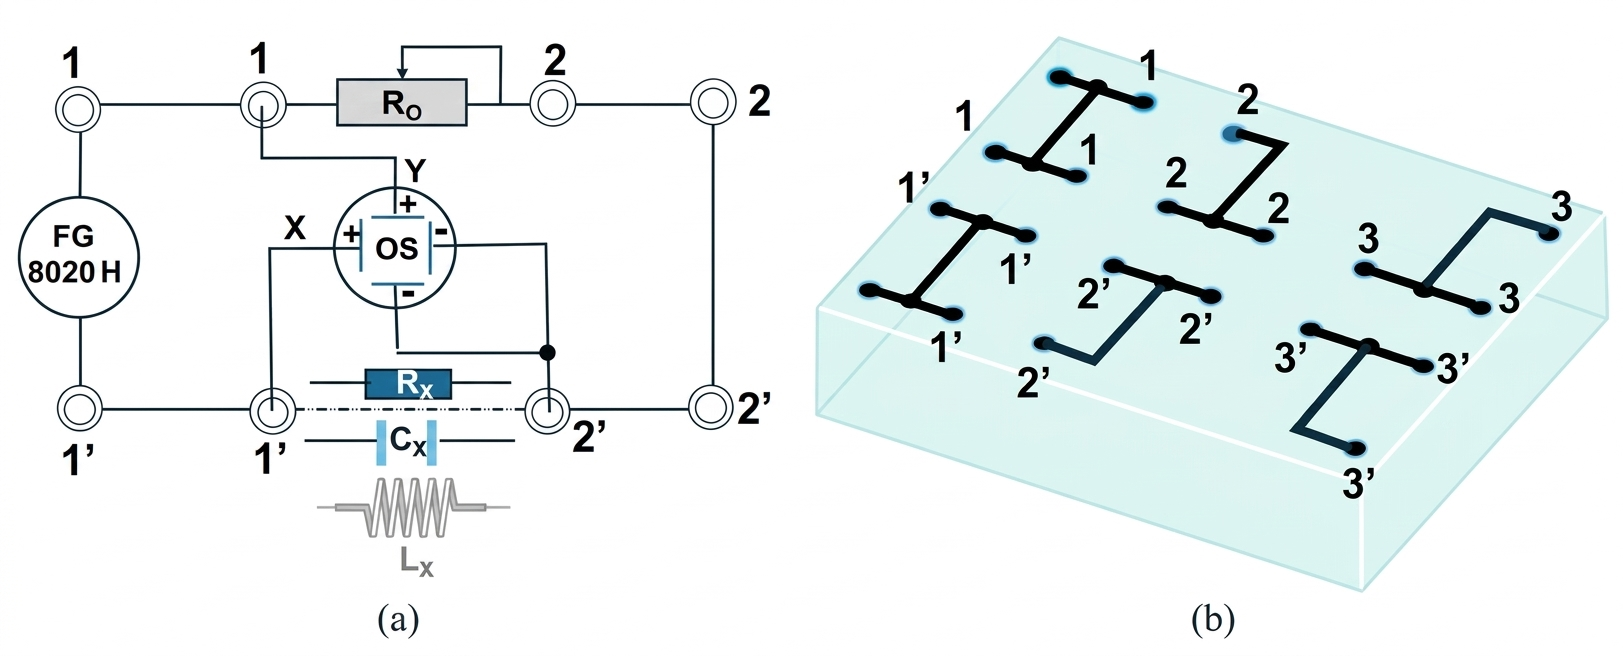
\includegraphics[width=\textwidth]{RLC measure}
		\captionof{figure}{\textit{ Measurement circuit layout (a), connection box with the notations (b)}}
	\end{center}
	\subsubsection*{2.1.1. Measurement of unknown resistance ($R_X$)}
	\begin{enumerate}[leftmargin=1.5em]
		\item Connect the Function Generator (FG) output to terminals $1$ and $1'$ of the connection box. Set FG to sine wave output at an initial frequency of $500\text{ Hz}$ (or $1000\text{ Hz}$).
		\item Connect the standard resistance box $R_0$ between points $1$ and $2$, the unknown resistor $R_X$ between points $1'$ and $2'$, and a U-shape connector between points $2$ and $2'$.
		\item Connect the OS X-channel to points $1'$ and $2'$, and the Y-channel to points $1$ and $2$. Center the trace on the OS screen.
		\item Adjust $R_0$ (from higher to lower decade knobs) until the vertical line becomes a diagonal line ($U_X = U_Y \implies R_X = R_0$). Record $f$ and $R_0$ in Table 1.
		\item Reset $R_0$ to zero and repeat the measurement for two additional frequencies (e.g., $1000\text{ Hz}$ and $1500\text{ Hz}$, or $1500\text{ Hz}$ and $2000\text{ Hz}$).
	\end{enumerate}
	
	\subsubsection*{2.1.2. Measurement of unknown capacitance ($C_X$)}
	\begin{enumerate}[leftmargin=1.5em]
		\item Replace $R_X$ with the unknown capacitor $C_X$ between points $1'$ and $2'$, and set FG frequency to $1000\text{ Hz}$.
		\item Center the upright oval trace on the OS screen and adjust $R_0$ until the oval becomes a circle. Record $f$ and $R_0$ in Table 2, then calculate $C_X$ using Eq. (11).
		\item Reset $R_0$ to zero and repeat for $2000\text{ Hz}$ and $3000\text{ Hz}$.
	\end{enumerate}
	
	\subsubsection*{2.1.3. Measurement of unknown inductance ($L_X$)}
	\begin{enumerate}[leftmargin=1.5em]
		\item Replace $C_X$ with the unknown coil $L_X$ between points $1'$ and $2'$, and set FG frequency to $10000\text{ Hz}$.
		\item Center the upright oval trace on the OS screen and adjust $R_0$ until the oval becomes a circle. Record $f$ and $R_0$ in Table 3, then calculate $L_X$ using Eq. (12).
		\item Reset $R_0$ to zero and repeat for $20000\text{ Hz}$ and $30000\text{ Hz}$.
	\end{enumerate}
	
	\subsection*{2.2. Measurement of Resonant Frequency of RLC Circuit}
	\subsubsection*{2.2.1. Parallel RLC circuit}
	\begin{enumerate}[leftmargin=1.5em]
		\item Connect $R_0$ ($1000\,\Omega$) between points $1$ and $2$. Insert U-shape connectors across $(2,3)$, $(2',3')$, and $(1',2')$. Connect both $C_X$ and $L_X$ in parallel across points $3$ and $3'$. Connect OS X-channel to $(1,1')$ and Y-channel to $(2,2')$.
		\item Adjust the FG frequency knobs until the oblique oval on the OS screen collapses into an inclined straight line. Record the parallel resonant frequency $f_p$ in Table 4.
		\item Repeat the measurement two more times to obtain three trials.
	\end{enumerate}
	\begin{figure}[H]
		\centering
		\begin{circuitikz}[american, line width=0.8pt]
			% Định nghĩa kiểu nút giắc cắm (vòng tròn đôi)
			\tikzset{
				jack/.style={draw, circle, inner sep=0pt, minimum size=12pt, fill=white,
					path picture={\draw (path picture bounding box.center) circle (3.5pt);}}
			}
			
			% 1. Khung dây nhánh trên: 1 -> 1 -> R_0 -> 2 -> 3 -> 3
			\draw (0,0) -- (0,4) -- (2.2,4)
			to[european potentiometer, l_=$R_0$] (5.8,4)
			-- (8.5,4) -- (11,4);
			
			% 2. Khung dây nhánh dưới: 1' -> 1' -> 2' -> 3' -> 3'
			\draw (0,0) -- (2.2,0) -- (5.8,0) -- (8.5,0) -- (11,0);
			
			% 3. Hai nhánh mắc song song: Tụ C_x (tại x=8.5) và Cuộn cảm L_x (tại x=11)
			\draw (8.5,4) to[C, l_=$C_x$] (8.5,0);
			\draw (11,4)  to[L, l=$L_x$]  (11,0);
			
			% 4. Máy phát tần số FG 8020 H (bên trái)
			\node[draw, circle, fill=white, minimum size=1.6cm, align=center, font=\bfseries\small] at (0,2) {FG\\8020 H};
			
			% 5. Dao động ký OS (gồm 4 bản cực lệch hướng và dấu +, -)
			\begin{scope}[shift={(4,2)}]
				\draw[fill=white] (0,0) circle (0.85cm);
				\node[font=\bfseries\small] at (0,0) {OS};
				% 4 bản cực bên trong
				\draw[thick] (-0.3, 0.42) -- (0.3, 0.42);   % Y+
				\draw[thick] (-0.3,-0.42) -- (0.3,-0.42);   % Y-
				\draw[thick] (-0.42,-0.3) -- (-0.42, 0.3);  % X+
				\draw[thick] ( 0.42,-0.3) -- ( 0.42, 0.3);  % X-
				% Dấu cực tính (+ / -)
				\node[font=\bfseries\scriptsize] at ( 0.25, 0.62) {+};
				\node[font=\bfseries\scriptsize] at ( 0.25,-0.62) {-};
				\node[font=\bfseries\scriptsize] at (-0.62, 0.25) {+};
				\node[font=\bfseries\scriptsize] at ( 0.62, 0.25) {-};
			\end{scope}
			
			% Dây nối từ các giắc cắm vào kênh X và Y của OS
			\draw (2.2,4) -- (2.2,2) -- (3.58,2);                  % Giắc 1 -> X+
			\node[font=\bfseries\small] at (3.0, 2.25) {X};
			
			\draw (5.8,4) -- (5.8,3.2) -- (4,3.2) -- (4,2.42);     % Giắc 2 -> Y+
			\node[font=\bfseries\small] at (3.65, 3.1) {Y};
			
			% Nối chung hai cực âm (X- và Y-) về giắc 2'
			\draw (4.42,2) -- (5.8,2) -- (5.8,0);                  % X- -> Giắc 2'
			\draw (4,1.58) -- (4,0.8) -- (5.8,0.8);                % Y- nối chung dây về 2'
			\fill (5.8,0.8) circle (2pt);                          % Chấm nối dây
			
			% 6. Vẽ tất cả các giắc cắm (vòng tròn đôi) đè lên trên dây và gắn nhãn
			\node[jack, label=above:{\textbf{1}}]  at (0,4) {};
			\node[jack, label=above:{\textbf{1}}]  at (2.2,4) {};
			\node[jack, label=above:{\textbf{2}}]  at (5.8,4) {};
			\node[jack, label=above:{\textbf{3}}]  at (8.5,4) {};
			\node[jack, label=above:{\textbf{3}}]  at (11,4) {};
			
			\node[jack, label=below:{\textbf{1'}}] at (0,0) {};
			\node[jack, label=below:{\textbf{1'}}] at (2.2,0) {};
			\node[jack, label=below:{\textbf{2'}}] at (5.8,0) {};
			\node[jack, label=below:{\textbf{3'}}] at (8.5,0) {};
			\node[jack, label=below:{\textbf{3'}}] at (11,0) {};
		\end{circuitikz}
		\caption{\textit{Parallel RLC circuit layout for measurement of resonant frequency}}
	\end{figure}
	
	\subsubsection*{2.2.2. Series RLC circuit}
	\begin{enumerate}[leftmargin=1.5em]
		\item Keep $R_0 = 1000\,\Omega$ across $(1,2)$ and U-shape connectors across $(2,3)$ and $(1',2')$. Move $C_X$ to points $(2',3')$ so that $C_X$ and $L_X$ (at $3,3'$) are connected in series. Keep OS connections unchanged.
		\item Vary the FG frequency until the oblique oval collapses into an inclined straight line. Record the series resonant frequency $f_s$ in Table 4.
		\item Repeat the measurement two more times to obtain three trials.
	\end{enumerate}
	\begin{figure}[H]
		\centering
		\begin{circuitikz}[american, line width=0.8pt]
			% Định nghĩa kiểu nút giắc cắm (vòng tròn đôi)
			\tikzset{
				jack/.style={draw, circle, inner sep=0pt, minimum size=12pt, fill=white,
					path picture={\draw (path picture bounding box.center) circle (3.5pt);}}
			}
			
			% 1. Khung dây nhánh trên: 1 -> 1 -> R_0 -> 2 -> 3 -> 3
			\draw (0,0) -- (0,4) -- (2.2,4)
			to[european potentiometer, l_=$R_0$] (5.8,4)
			-- (8.5,4) -- (11,4);
			
			% 2. Khung dây nhánh dưới: 1' -> 1' -> 2' -> C_x -> 3' -> 3'
			\draw (0,0) -- (2.2,0) -- (5.8,0)
			to[C, l=$C_x$] (8.5,0)
			-- (11,0);
			
			% 3. Nhánh cuộn cảm L_x mắc nối tiếp ở bên phải (giữa 3 và 3')
			\draw (11,4) to[L, l=$L_x$] (11,0);
			
			% 4. Máy phát tần số FG 8020 H (bên trái)
			\node[draw, circle, fill=white, minimum size=1.6cm, align=center, font=\bfseries\small] at (0,2) {FG\\8020 H};
			
			% 5. Dao động ký OS (gồm 4 bản cực lệch hướng và dấu +, -)
			\begin{scope}[shift={(4,2)}]
				\draw[fill=white] (0,0) circle (0.85cm);
				\node[font=\bfseries\small] at (0,0) {OS};
				% 4 bản cực bên trong
				\draw[thick] (-0.3, 0.42) -- (0.3, 0.42);   % Y+
				\draw[thick] (-0.3,-0.42) -- (0.3,-0.42);   % Y-
				\draw[thick] (-0.42,-0.3) -- (-0.42, 0.3);  % X+
				\draw[thick] ( 0.42,-0.3) -- ( 0.42, 0.3);  % X-
				% Dấu cực tính (+ / -)
				\node[font=\bfseries\scriptsize] at ( 0.25, 0.62) {+};
				\node[font=\bfseries\scriptsize] at ( 0.25,-0.62) {-};
				\node[font=\bfseries\scriptsize] at (-0.62, 0.25) {+};
				\node[font=\bfseries\scriptsize] at ( 0.62, 0.25) {-};
			\end{scope}
			
			% Dây nối từ các giắc cắm vào kênh X và Y của OS
			\draw (2.2,4) -- (2.2,2) -- (3.58,2);                  % Giắc 1 -> X+
			\node[font=\bfseries\small] at (3.0, 2.25) {X};
			
			\draw (5.8,4) -- (5.8,3.2) -- (4,3.2) -- (4,2.42);     % Giắc 2 -> Y+
			\node[font=\bfseries\small] at (3.65, 3.1) {Y};
			
			% Nối chung hai cực âm (X- và Y-) về giắc 2'
			\draw (4.42,2) -- (5.8,2) -- (5.8,0);                  % X- -> Giắc 2'
			\draw (4,1.58) -- (4,0.8) -- (5.8,0.8);                % Y- nối chung dây về 2'
			\fill (5.8,0.8) circle (2pt);                          % Chấm nối dây
			
			% 6. Vẽ tất cả các giắc cắm (vòng tròn đôi) đè lên trên dây và gắn nhãn
			\node[jack, label=above:{\textbf{1}}]  at (0,4) {};
			\node[jack, label=above:{\textbf{1}}]  at (2.2,4) {};
			\node[jack, label=above:{\textbf{2}}]  at (5.8,4) {};
			\node[jack, label=above:{\textbf{3}}]  at (8.5,4) {};
			\node[jack, label=above:{\textbf{3}}]  at (11,4) {};
			
			\node[jack, label=below:{\textbf{1'}}] at (0,0) {};
			\node[jack, label=below:{\textbf{1'}}] at (2.2,0) {};
			\node[jack, label=below:{\textbf{2'}}] at (5.8,0) {};
			\node[jack, label=below:{\textbf{3'}}] at (8.5,0) {};
			\node[jack, label=below:{\textbf{3'}}] at (11,0) {};
		\end{circuitikz}
		\caption{\textit{Series RLC circuit layout for measurement of resonant frequency}}
	\end{figure}
	
	\section*{3. EXPERIMENTAL RESULTS}
	\subsection*{3.1. Measurement of resistance, capacitance, and inductance}
	\subsubsection*{3.1.1. Data Tables}
	
	\begin{table}[H]
		\centering
		\caption{Measurement of unknown resistance $R_X$}
		\begin{tabular}{|>{\centering\arraybackslash}m{1.5cm}|>{\centering\arraybackslash}m{4.5cm}|>{\centering\arraybackslash}m{5.5cm}|}
			\hline
			\textbf{Trial} & \textbf{Frequency $f$ (Hz)} & \textbf{Standard Resistance $R_0$ ($\Omega$)} \rule[-0.2cm]{0pt}{0.6cm} \\
			\hline
			1 & 500 & 560 \rule[-0.25cm]{0pt}{0.7cm} \\
			\hline
			2 & 1000 & 557 \rule[-0.25cm]{0pt}{0.7cm} \\
			\hline
			3 & 1500 & 562 \rule[-0.25cm]{0pt}{0.7cm} \\
			\hline
		\end{tabular}
	\end{table}
	
	\begin{table}[H]
		\centering
		\caption{Measurement of unknown capacitance $C_X$}
		\begin{tabular}{|>{\centering\arraybackslash}m{1.5cm}|>{\centering\arraybackslash}m{4.5cm}|>{\centering\arraybackslash}m{5.5cm}|}
			\hline
			\textbf{Trial} & \textbf{Frequency $f$ (Hz)} & \textbf{Standard Resistance $R_0$ ($\Omega$)} \rule[-0.2cm]{0pt}{0.6cm} \\
			\hline
			1 & 1000 & 251  \rule[-0.25cm]{0pt}{0.7cm} \\
			\hline
			2 & 2000 & 133  \rule[-0.25cm]{0pt}{0.7cm} \\
			\hline
			3 & 3000 & 81  \rule[-0.25cm]{0pt}{0.7cm} \\
			\hline
		\end{tabular}
	\end{table}
	
	\begin{table}[H]
		\centering
		\caption{Measurement of unknown inductance $L_X$}
		\begin{tabular}{|>{\centering\arraybackslash}m{1.5cm}|>{\centering\arraybackslash}m{4.5cm}|>{\centering\arraybackslash}m{5.5cm}|}
			\hline
			\textbf{Trial} & \textbf{Frequency $f$ (Hz)} & \textbf{Standard Resistance $R_0$ ($\Omega$)} \rule[-0.2cm]{0pt}{0.6cm} \\
			\hline
			1 & 10007 & 60 \rule[-0.25cm]{0pt}{0.7cm} \\
			\hline
			2 & 20009 & 120 \rule[-0.25cm]{0pt}{0.7cm} \\
			\hline
			3 & 30004 & 161 \rule[-0.25cm]{0pt}{0.7cm} \\
			\hline
		\end{tabular}
	\end{table}
	
	\subsubsection*{3.1.2. Data processing}
	\textbf{{\normalsize For unknown resistance $R_X$}}
	
	\noindent	
	Since the traces obtained after 3 trials are diagonal lines, $U_X = U_Y = U_{R_0}, \text{ implying that } R_X = R_0$. Hence, the mean value of unknown resistance is
	\begin{center}
		\fbox{%
			\begin{minipage}{0.8\textwidth}
				\vspace{-0.4cm}
				\centering
				\begin{displaymath}
					\overline{R_X} = \frac{R_{X1} + R_{X2} + R_{X3}}{3} = \dfrac{560 + 557 + 562}{3} = \dfrac{1679}{3} \approx 559.667 \left(\Omega\right)
				\end{displaymath}
			\end{minipage}%
		}
	\end{center}
	
	\noindent
	The standard deviation of a single measurement is
	\begin{center}
	\fbox{%
		\begin{minipage}{0.8\textwidth}
			\vspace{-0.4cm}
			\centering
			\begin{displaymath}
				\text{sd} = \sqrt{\frac{\left(R_{X1} - \overline{R_X}\right)^2 + \left(R_{X2} - \overline{R_X}\right)^2 + \left(R_{X3} - \overline{R_X}\right)^2}{3}} = \dfrac{\sqrt{38}}{3} \left(\Omega\right)
			\end{displaymath}
		\end{minipage}%
	}
	\end{center}
	
	\noindent
	And the standard deviation of the mean is
	\begin{center}
	\fbox{%
		\begin{minipage}{0.8\textwidth}
			\vspace{-0.4cm}
			\centering
			\begin{displaymath}
				\text{SD} = \dfrac{\text{sd}}{\sqrt{3}} = \dfrac{\sqrt{114}}{9} \approx 1.186 \left(\Omega\right)
			\end{displaymath}
		\end{minipage}%
	}
	\end{center}
	
	\noindent
	Therefore, our result for $R_X$ appears as
	\begin{center}
	\fbox{%
		\begin{minipage}{0.8\textwidth}
			\vspace{-0.4cm}
			\centering
			\begin{displaymath}
				R_X = \overline{R_X} \pm \text{SD} = 559.667 \pm 1.186 \left(\Omega\right)
			\end{displaymath}
		\end{minipage}%
	}
	\end{center}			
	
	\noindent
	\textbf{For unknown capacitance $C_X$}
	
	\noindent
	Since the traces obtained after 3 trials are circles, $C_X = \frac{1}{2\pi f R_0}$. Hence, we have
	\begin{center}
	\fbox{%
		\begin{minipage}{0.8\textwidth}
			\vspace{-0.4cm}
			\centering
			\begin{displaymath}
				\begin{aligned}
					&C_{X1} = \dfrac{1}{2 \pi \times 1000 \times 251} \approx 6.341 \times 10^{-7} \left(\text{F}\right)\\
					&C_{X2} = \dfrac{1}{2 \pi \times 2000 \times 133} \approx 5.983 \times 10^{-7} \left(\text{F}\right)\\
					&C_{X3} = \dfrac{1}{2 \pi \times 3000 \times 81} \approx 6.550 \times 10^{-7} \left(\text{F}\right)
				\end{aligned}
			\end{displaymath}
		\end{minipage}%
	}
	\end{center}
	
	\noindent
	The mean value of unknown capacitance is
	\begin{center}
		\fbox{%
			\begin{minipage}{0.8\textwidth}
				\vspace{-0.4cm}
				\centering
				\begin{displaymath}
					\overline{C_X} = \frac{C_{X1} + C_{X2} + C_{X3}}{3} \approx \dfrac{6.341 + 5.983 + 6.550}{3} \times 10^{-7} \approx 6.291 \times 10^{-7} \left(\text{F}\right)
				\end{displaymath}
			\end{minipage}%
		}
	\end{center}
		
	\noindent
	The standard deviation of a single measurement is
	\begin{center}
		\fbox{%
			\begin{minipage}{0.8\textwidth}
				\vspace{-0.4cm}
				\centering
				\begin{displaymath}
					\text{sd} = \sqrt{\frac{\left(C_{X1} - \overline{C_X}\right)^2 + \left(C_{X2} - \overline{C_X}\right)^2 + \left(C_{X3} - \overline{C_X}\right)^2}{3}} \approx 0.234 \times 10^{-7} \left(\text{F}\right)
				\end{displaymath}
			\end{minipage}%
		}
	\end{center}
	
	\noindent
	And the standard deviation of the mean is
	\begin{center}
		\fbox{%
			\begin{minipage}{0.8\textwidth}
				\vspace{-0.4cm}
				\centering
				\begin{displaymath}
					\text{SD} = \dfrac{\text{sd}}{\sqrt{3}} \approx 0.135 \times 10^{-7} \left(\text{F}\right)
				\end{displaymath}
			\end{minipage}%
		}
	\end{center}
	
	\noindent
	Therefore, our result for $C_X$ appears as
	\begin{center}
		\fbox{%
			\begin{minipage}{0.8\textwidth}
				\vspace{-0.4cm}
				\centering
				\begin{displaymath}
					C_X = \overline{C_X} \pm \text{SD} = \left(6.291 \pm 0.135\right) \times 10^{-7} \left(\text{F}\right)
				\end{displaymath}
			\end{minipage}%
		}
	\end{center}
		
	\noindent
	\textbf{For unknown inductance $L_X$}
	
	\noindent
	Since the traces obtained after 3 trials are circles, $L_X = \frac{R_0}{2\pi f}$. Hence, we have
	\begin{center}
		\fbox{%
			\begin{minipage}{0.8\textwidth}
				\vspace{-0.4cm}
				\centering
				\begin{displaymath}
					\begin{aligned}
						&L_{X1} = \dfrac{60}{2 \pi \times 100007} \approx 9.543\times 10^{-4} \left(\text{H}\right)\\
						&L_{X2} = \dfrac{120}{2 \pi \times 20009} \approx 9.545 \times 10^{-4} \left(\text{H}\right)\\
						&L_{X3} = \dfrac{161}{2 \pi \times 30004} \approx 8.540 \times 10^{-4} \left(\text{H}\right)
					\end{aligned}
				\end{displaymath}
			\end{minipage}%
		}
	\end{center}
	
	\noindent
	The mean value of unknown inductance is
	\begin{center}
		\fbox{%
			\begin{minipage}{0.8\textwidth}
				\vspace{-0.4cm}
				\centering
				\begin{displaymath}
					\overline{L_X} = \frac{L_{X1} + L_{X2} + L_{X3}}{3} \approx \dfrac{9.543 + 9.545 + 8.540}{3} \times 10^{-4} \approx 9.209 \times 10^{-4} \left(\text{H}\right)
				\end{displaymath}
			\end{minipage}%
		}
	\end{center}
	
	\noindent
	The standard deviation of a single measurement is
	\begin{center}
		\fbox{%
			\begin{minipage}{0.8\textwidth}
				\vspace{-0.4cm}
				\centering
				\begin{displaymath}
					\text{sd} = \sqrt{\frac{\left(L_{X1} - \overline{L_X}\right)^2 + \left(L_{X2} - \overline{L_X}\right)^2 + \left(L_{X3} - \overline{L_X}\right)^2}{3}} \approx 0.473 \times 10^{-4} \left(\text{H}\right)
				\end{displaymath}
			\end{minipage}%
		}
	\end{center}
	
	\noindent
	And the standard deviation of the mean is
	\begin{center}
		\fbox{%
			\begin{minipage}{0.8\textwidth}
				\vspace{-0.4cm}
				\centering
				\begin{displaymath}
					\text{SD} = \dfrac{\text{sd}}{\sqrt{3}} \approx 0.273 \times 10^{-4} \left(\text{H}\right)
				\end{displaymath}
			\end{minipage}%
		}
	\end{center}
	
	\noindent
	Therefore, our result for $L_X$ appears as
	\begin{center}
		\fbox{%
			\begin{minipage}{0.8\textwidth}
				\vspace{-0.4cm}
				\centering
				\begin{displaymath}
					L_X = \overline{L_X} \pm \text{SD} = \left(9.209 \pm 0.273\right) \times 10^{-4} \left(\text{H}\right)
				\end{displaymath}
			\end{minipage}%
		}
	\end{center}
	
	\subsection*{3.2. Resonant Frequencies of Parallel and Series RLC Circuits}
	\subsubsection*{3.2.1. Data table}
	\begin{table}[H]
		\centering
		\caption{Measurement of parallel and series resonant frequencies}
		\begin{tabular}{|>{\centering\arraybackslash}m{1.5cm}|>{\centering\arraybackslash}m{7cm}|>{\centering\arraybackslash}m{7cm}|}
			\hline
			\textbf{Trial} & \textbf{Parallel Resonant Frequency $f_p$ (Hz)} & \textbf{Series Resonant Frequency $f_s$ (Hz)} \rule[-0.2cm]{0pt}{0.6cm} \\
			\hline
			1 & 6568 & 6421 \rule[-0.25cm]{0pt}{0.7cm} \\
			\hline
			2 & 6570 & 6725 \rule[-0.25cm]{0pt}{0.7cm} \\
			\hline
			3 & 6572 & 6750 \rule[-0.25cm]{0pt}{0.7cm} \\
			\hline
		\end{tabular}
	\end{table}
	\subsubsection*{3.2.2. Data processing}
	
	\noindent
	The mean values of parallel resonant frequency and series resonant frequency are
	\begin{center}
		\fbox{%
			\begin{minipage}{0.8\textwidth}
				\vspace{-0.4cm}
				\centering
				\begin{displaymath}
					\begin{aligned}
						&\overline{f_p} = \frac{f_{p1} + f_{p2} + f_{p3}}{3} = \dfrac{6568 + 6570 + 6572}{3} = 6570 \left(\text{Hz}\right) \\
						&\overline{f_s} = \frac{f_{s1} + f_{s2} + f_{s3}}{3} = \dfrac{6421 + 6725 + 6750}{3} = 6632 \left(\text{Hz}\right)
					\end{aligned}
				\end{displaymath}
			\end{minipage}%
		}
	\end{center}
	
	\noindent
	The standard deviations of a single measurement for $f_p$ and $f_s$ are
	\begin{center}
		\fbox{%
			\begin{minipage}{0.8\textwidth}
				\vspace{-0.4cm}
				\centering
				\begin{displaymath}
					\begin{aligned}
						&\text{sd}_{f_p} = \sqrt{\frac{\left(f_{p1} - \overline{f_p}\right)^2 + \left(f_{p2} - \overline{f_p}\right)^2 + \left(f_{p3} - \overline{f_p}\right)^2}{3}} = \dfrac{2\sqrt{6}}{3} \left(\text{Hz}\right) \\
						&\text{sd}_{f_s} = \sqrt{\frac{\left(f_{s1} - \overline{f_s}\right)^2 + \left(f_{s2} - \overline{f_s}\right)^2 + \left(f_{s3} - \overline{f_s}\right)^2}{3}} \approx 149.548 \left(\text{Hz}\right)
					\end{aligned}
				\end{displaymath}
			\end{minipage}%
		}
	\end{center}
	
	\noindent
	And the standard deviations of the means for $f_p$ and $f_s$ are
	\begin{center}
		\fbox{%
			\begin{minipage}{0.8\textwidth}
				\vspace{-0.4cm}
				\centering
				\begin{displaymath}
					\begin{aligned}
						&\text{SD}_{f_p} = \dfrac{\text{sd}_{f_p}}{\sqrt{3}} \approx 0.943 \left(\text{Hz}\right) \\
						&\text{SD}_{f_s} = \dfrac{\text{sd}_{f_s}}{\sqrt{3}} \approx 86.342 \left(\text{Hz}\right)
					\end{aligned}
				\end{displaymath}
			\end{minipage}%
		}
	\end{center}
	
	\noindent
	Therefore, our result for $f_p$ and $f_s$ appear as
	\begin{center}
		\fbox{%
			\begin{minipage}{0.8\textwidth}
				\vspace{-0.4cm}
				\centering
				\begin{displaymath}
					\begin{aligned}
						&f_p = \overline{f_p} \pm \text{SD}_{f_p} = 6570.000 \pm 0.943 \left(\text{Hz}\right) \\
						&f_s = \overline{f_s} \pm \text{SD}_{f_s} = 6632.000 \pm 86.342 \left(\text{Hz}\right)
					\end{aligned}
				\end{displaymath}
			\end{minipage}%
		}
	\end{center}
	
	\begin{bt}
		\textit{Compare the measured average values of parallel ($\overline{f}_p$) and series ($\overline{f}_s$) resonant frequencies with the theoretical resonant frequency $f_0$ calculated using Eq. (2), and discuss sources of experimental error.}
		
		\vspace{0.2cm}
		\noindent
		From Eq. (2), the theoretical mean resonant frequency calculated from $\overline{L_X}$ and $\overline{C_X}$ is
		\begin{center}
			\fbox{%
				\begin{minipage}{0.8\textwidth}
					\vspace{-0.4cm}
					\centering
					\begin{displaymath}
						\overline{f_0} = \frac{1}{2\pi \sqrt{\overline{L}_X \overline{C}_X}} 
						= \dfrac{1}{2\pi \sqrt{\left(9.209 \times 10^{-4}\right) \times \left(6.291 \times 10^{-7}\right)}} \approx 6612.323 
						\left(\text{Hz}\right)
					\end{displaymath}
				\end{minipage}%
			}
		\end{center}
		
		\noindent
		By the propagation of uncertainty, the relative uncertainty in $\overline{f_0}$ is
		\begin{center}
			\fbox{%
				\begin{minipage}{0.8\textwidth}
					\vspace{-0.4cm}
					\centering
					\begin{displaymath}
						\dfrac{\Delta f_0}{\overline{f_0}} = \sqrt{\left(\dfrac{-1}{2} \times \dfrac{\Delta L_X}{\overline{L_X}}\right)^2 + \left(\dfrac{-1}{2} \times \dfrac{\Delta C_X}{\overline{C_X}}\right)^2} = \dfrac{1}{2} \times \sqrt{\left(\dfrac{\Delta L_X}{\overline{L_X}}\right)^2 + \left(\dfrac{\Delta C_X}{\overline{C_X}}\right)^2}
					\end{displaymath}
				\end{minipage}%
			}
		\end{center}
		
		\noindent
		And the uncertainty in $f_0$ is
		\begin{center}
			\fbox{%
				\begin{minipage}{0.8\textwidth}
					\vspace{-0.4cm}
					\centering
					\begin{displaymath}
						\Delta f_0 = \dfrac{\overline{f_0}}{2} \times \sqrt{\left(\dfrac{\Delta L_X}{\overline{L_X}}\right)^2 + \left(\dfrac{\Delta C_X}{\overline{C_X}}\right)^2} \approx 120.995 \left(\text{Hz}\right)
					\end{displaymath}
				\end{minipage}%
			}
		\end{center}
		
		\noindent
		Therefore, the theoretical resonant frequency $f_0$ is
		\begin{center}
			\fbox{%
				\begin{minipage}{0.8\textwidth}
					\vspace{-0.4cm}
					\centering
					\begin{displaymath}
						f_0 = \overline{f_0} \pm \Delta f_0 = 6612.323 \pm 120.995 \left(\text{Hz}\right)
					\end{displaymath}
				\end{minipage}%
			}
		\end{center}
		
		\noindent
		The measured average resonant frequencies $\overline{f}_p$ and $\overline{f}_s$ are in close agreement with the theoretical value $f_0 = \frac{1}{2\pi\sqrt{\overline{L}_X \overline{C}_X}}$. Any slight discrepancies arise from the non-zero internal ohmic resistance of the inductor coil (which shifts the damped parallel resonant frequency slightly below $f_0$), parasitic capacitance and inductance in the connecting wires, and visual judgment uncertainty when determining the exact collapse of the Lissajous ellipse into a straight line on the oscilloscope screen.
	\end{bt}
	
\end{document}
